\subsection{区间上的问题}

\subsubsection{选择不相交区间}
	\paragraph{问题} 数轴上有 $n$ 个开区间  $(a_i,b_i)$。选择尽量多的区间,使这些区间两两没有公共点。
	
	\paragraph{思路} 贪心策略如下:
	
	\begin{enumerate}
		\item 按 $b_i$ 从小到大的顺序排序。
		\item 务必选择第一个区间。(原因见图 \ref{fig:ch1_tx_qjsdwt_1})
		\item 继续从前向后遍历。每当遇到可以选择的区间(与上一区间没有公共点),就选择它。
	\end{enumerate}
	
	\begin{figure}[htb]
		\centering
		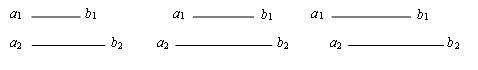
\includegraphics{ch1/figures/选择不相交区间.png}
		\label{fig:ch1_tx_qjsdwt_1}
		\caption{选择不相交区间:如图所示,不论区间 1、2 的相对位置如何,选择区间 1 都会为以后的选择留下更大的剩余空间。}
	\end{figure}

\subsubsection{区间选点问题}
	\paragraph{问题} 数轴上有 $n$ 个闭区间 $[a_i, b_i]$。取尽量少的点,使得每个区间内都至少有一个点(不同区间内含有的点可以是同一个)。
	
	\paragraph{思路} 贪心策略如下:
	
	\begin{enumerate}
		\item 把所有区间按 $b_i$ 从小到大排序($b_i$ 相同时,$a$ 从大到小排序\footnote{考虑区间包含的情况:小区间被满足时大区间一定被满足。所以我们应当优先选取小区间中的点,这样大区间不必考虑。})。
		\item 然后,一定取第一个区间的右端点。(原因见图 \ref{fig:ch1_tx_qjsdwt_2})
		\item 继续从前向后遍历,当遇到覆盖不到的区间时,选取这个区间的右端点。
	\end{enumerate}
	
	\begin{figure}[htb]
		\centering
		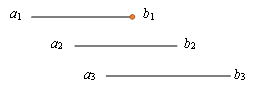
\includegraphics{ch1/figures/区间选点问题.png}
		\label{fig:ch1_tx_qjsdwt_2}
		\caption{区间选点问题:对于第 1 个区间来说,显然,选择它的右端点是明智的。因为它比前面的点能覆盖更大的范围。}
	\end{figure}

\subsubsection{区间覆盖问题}
	\paragraph{问题} 数轴上有 $n$ 个闭区间 $[a_i, b_i]$。选择尽量少的区间来覆盖指定线段 $[s, t]$。

	\paragraph{思路} 贪心策略如下:
	
	\begin{enumerate}
		\item 预处理,扔掉不能覆盖 $[s, t]$ 的区间。如果区间边界超过了 $[s, t]$,就把它变成 $s$ 或 $t$,以免影响后面的处理。
		\item 把各区间按 $a$ 从小到大排序。如果区间 1 的起点不是 $s$,无解,否则选择起点在 $s$ 的最长区间。
		\item 选择此区间 $[a_i, b_i]$ 后,问题就转化成了起点为 $b_i$ 的区间 $[b_i, t]$。继续选择,直到找不到区间覆盖当前起点,或者 $b_i$ 已经到达线段末端。
	\end{enumerate}
	
	
	